\documentclass[a4paper,11pt,fleqn]{article}		% Présentation générale et mise en page


\input{preambule}
\input{preambule-partages}
\input{preambule-axes-gradues}


%\input{preambule}
\setlength{\columnsep}{1cm}
\setlength{\columnseprule}{.5pt}


\renewcommand{\headrulewidth}{1pt}
\fancyhead[C]{\textbf{Entraînement -- Calcul littéral niveau 1 version \no <<version>>}} 
\fancyhead[L]{}
\fancyhead[R]{Cycle 4}

\renewcommand{\footrulewidth}{1pt}
\fancyfoot[C]{} 
\fancyfoot[L]{}
\fancyfoot[R]{Calcul littéral niveau 1}


\usepackage{titlesec}
\titlespacing*{\subsection}
{1pt}{.1ex plus 0.1ex minus .1ex}{.1ex plus .1ex}

\begin{document}

\setcounter{exo}{0}
\vfill
\begin{correction}
\begin{multicols}{2}
%
%\exo{}
%
%\begin{enumerate}
%	\item $2z$
%	\item $3z$
%	\item $\frac{z}{2}$
%	\item $7z$
%	\item $5z+2z=7z$
%	\item $2(5+z)$
%\end{enumerate}

\exo{ - Version 1.0}

Programme 1 : $-7 x +4$\\
Programme 2 : $(x +3)\times (-7)= -7  x  -21 $\\
Programme 3 : $( 8 x -2 )\times 2= 16 x -4$

\exo{ - Version 2.0}

Programme 1 : $-5 x +9$\\
Programme 2 : $(x -2)\times 9= 9  x  -18 $\\
Programme 3 : $( 2 x -5 )\times 2= 4 x -10$

\exo{ - Version 3.0}

Programme 1 : $-8 x +2$\\
Programme 2 : $(x -2)\times (-7)= -7  x  +14 $\\
Programme 3 : $( 2 x +9 )\times 2= 4 x +18$

\exo{ - Version 4.0}

Programme 1 : $-3 x -8$\\
Programme 2 : $(x -2)\times 2= 2  x  -4 $\\
Programme 3 : $( 4 x -4 )\times 2= 8 x -8$

\exo{ - Version 1.0}

%Simplifier les expressions suivantes.

%\begin{multicols}{2}
$A=(6  +2) x=8 x$\\
$B=-7 \times x\times x=-7 \times x^2$\\
$C=(7 +9) \times x=16  x$\\
$D=7\times 9\times x\times x=63\times x^2$\\
$E= 2  x +5 x -3\times (-9) = (2  +5) x +27 = 7 x +27 $\\
$F=7 \times (-5y -9)  =7 \times (-5)y +7 \times (-9)
 =-35y -63 $\\
$G=2 a^2+a\times (2+ 1)=2 a^2+3a$\\
$H= (3 -6)x = (-3)x$
%\end{multicols}
\exo{ - Version 2.0}

%Simplifier les expressions suivantes.

%\begin{multicols}{2}
$A=(9  +8) x=17 x$\\
$B=4 \times x\times x=4 \times x^2$\\
$C=(6 +3) \times x=9  x$\\
$D=6\times 3\times x\times x=18\times x^2$\\
$E= 3  x +7 x -3\times 9 = (3  +7) x -27 = 10 x -27 $\\
$F=-8 \times (-3y -2)  =-8 \times (-3)y -8 \times (-2)
 =24y +16 $\\
$G=2 a^2+a\times (1+ 1)=2 a^2+2a$\\
$H= (2 -6)x = (-4)x$
%\end{multicols}
\exo{ - Version 3.0}

%Simplifier les expressions suivantes.

%\begin{multicols}{2}
$A=(9  +5) x=14 x$\\
$B=-3 \times x\times x=-3 \times x^2$\\
$C=(-5 -5) \times x=-10  x$\\
$D=-5\times (-5)\times x\times x=25\times x^2$\\
$E= -9  x -9 x +2\times (-7) = (-9  -9) x -14 = -18 x -14 $\\
$F=-7 \times (8y +7)  =-7 \times 8y -7 \times 7
 =-56y -49 $\\
$G=2 a^2+a\times (2+ 3)=2 a^2+5a$\\
$H= (2 +8)x = (10)x$
%\end{multicols}
\exo{ - Version 4.0}

%Simplifier les expressions suivantes.

%\begin{multicols}{2}
$A=(3  +6) x=9 x$\\
$B=-8 \times x\times x=-8 \times x^2$\\
$C=(3 +6) \times x=9  x$\\
$D=3\times 6\times x\times x=18\times x^2$\\
$E= 6  x -8 x +7\times 3 = (6  -8) x +21 = -2 x +21 $\\
$F=9 \times (3y +3)  =9 \times 3y +9 \times 3
 =27y +27 $\\
$G=1 a^2+a\times (1+ 3)=1 a^2+4a$\\
$H= (8 +2)x = (10)x$
%\end{multicols}
\exo{ - Version 1.0}
%Développer et réduire les expressions suivantes.
%\begin{multicols}{2}
$A=  5 (x  -6)=  5 x +5 \times (-6)=  5 x -30$\\
$B= 7 ( 7 x    +4)= 7 \times 7 x  +7 \times  4= 49 x  +28$\\
$C=y( -2  +2 y)=y \times (-2) + y \times 2 y=-2 y + 2 y^2$\\
$D= 2  t(  -2 t -5)= 2  t \times (-2) t +2  t \times (-5) = -4  t^2  -10  t  $
%\end{multicols}
\exo{ - Version 2.0}
%Développer et réduire les expressions suivantes.
%\begin{multicols}{2}
$A=  5 (x  +6)=  5 x +5 \times 6=  5 x +30$\\
$B= 9 ( 5 x    +2)= 9 \times 5 x  +9 \times  2= 45 x  +18$\\
$C=y( 3  -4 y)=y \times 3 + y \times -4 y=3 y + -4 y^2$\\
$D= 2  t(  3 t -7)= 2  t \times 3 t +2  t \times (-7) = 6  t^2  -14  t  $
%\end{multicols}
\exo{ - Version 3.0}
%Développer et réduire les expressions suivantes.
%\begin{multicols}{2}
$A=  -2 (x  -3)=  -2 x -2 \times (-3)=  -2 x +6$\\
$B= -2 ( -8 x    -3)= -2 \times (-8) x  -2 \times  (-3)= 16 x  +6$\\
$C=y( -2  +8 y)=y \times (-2) + y \times 8 y=-2 y + 8 y^2$\\
$D= 2  t(  -3 t -2)= 2  t \times (-3) t +2  t \times (-2) = -6  t^2  -4  t  $
%\end{multicols}
\exo{ - Version 4.0}
%Développer et réduire les expressions suivantes.
%\begin{multicols}{2}
$A=  -7 (x  +5)=  -7 x -7 \times 5=  -7 x -35$\\
$B= -2 ( 8 x    +3)= -2 \times 8 x  -2 \times  3= -16 x  -6$\\
$C=y( 2  +7 y)=y \times 2 + y \times 7 y=2 y + 7 y^2$\\
$D= 3  t(  8 t +4)= 3  t \times 8 t +3  t \times 4 = 24  t^2  +12  t  $
%\end{multicols}
\exo{ - Version 1.0}

Factoriser les expressions suivantes.

%\begin{multicols}{2}
$E=  7x \times 6   -1 \times  6 =   (7  x  -1 ) \times 6 $\\
$F=  -18  x  +6  x=  (-18   +6 ) \times  x=  -12  x$\\
$G=  -2 \times  x  +2 x\times x=  (-2   +2 x) \times  x$\\
$H=  -3 x^2  -9 x^2=  (-3 -9) x^2=  -12 x^2$
%\end{multicols}
\exo{ - Version 2.0}

Factoriser les expressions suivantes.

%\begin{multicols}{2}
$E=  3x \times 9   +1 \times  9 =   (3  x  +1 ) \times 9 $\\
$F=  42  x  +7  x=  (42   +7 ) \times  x=  49  x$\\
$G=  -36 \times  x  +9 x\times x=  (-36   +9 x) \times  x$\\
$H=  -2 x^2  +3 x^2=  (-2 +3) x^2=  1 x^2$
%\end{multicols}
\exo{ - Version 3.0}

Factoriser les expressions suivantes.

%\begin{multicols}{2}
$E=  9x \times 9   -1 \times  9 =   (9  x  -1 ) \times 9 $\\
$F=  24  x  +4  x=  (24   +4 ) \times  x=  28  x$\\
$G=  -3 \times  x  +3 x\times x=  (-3   +3 x) \times  x$\\
$H=  3 x^2  +6 x^2=  (3 +6) x^2=  9 x^2$
%\end{multicols}
\exo{ - Version 4.0}

Factoriser les expressions suivantes.

%\begin{multicols}{2}
$E=  8x \times 3   +1 \times  3 =   (8  x  +1 ) \times 3 $\\
$F=  -35  x  +5  x=  (-35   +5 ) \times  x=  -30  x$\\
$G=  32 \times  x  +8 x\times x=  (32   +8 x) \times  x$\\
$H=  5 x^2  +8 x^2=  (5 +8) x^2=  13 x^2$
%\end{multicols}
\end{multicols}

\exon{}

\begin{minipage}{0.4\linewidth}
	\begin{center}
	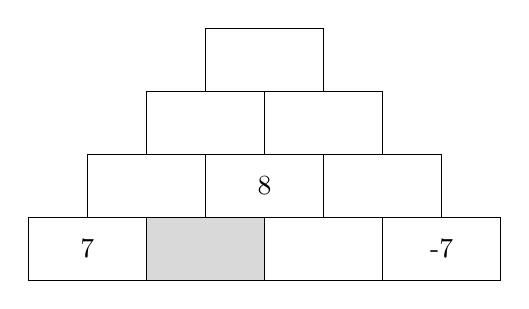
\begin{tikzpicture}
		\tikzstyle{brique}=[minimum width=1.5cm, minimum height=0.8cm,draw]
		\tikzstyle{brique_grise}=[minimum width=1.5cm, minimum height=0.8cm,draw,fill=gray!30]
		\node[brique] at (0,0) {  7 }; % gauche
		\node[brique_grise] at (1.5,0) {};
		\node[brique] at (3,0) {};
		\node[brique] at (4.5,0) { -7 };  % droite
		\node[brique] at (.75,.8) {};
		\node[brique] at (2.25,.8) {  8 };  % milieu bas
		\node[brique] at (3.75,.8) {};
		\node[brique] at (1.5,1.6) {};
		\node[brique] at (3,1.6) {};
		\node[brique] at (2.25,2.4) {};
	\end{tikzpicture} 	
\end{center}
\end{minipage}
\begin{minipage}{0.2\linewidth}
%Pour compléter cette pyramide, le nombre situé dans une case est la somme des deux nombres situés en dessous de lui.

\begin{enumerate}
	\item Fait à gauche.
	\item On peut mettre un nombre $x$ quelconque dans la case grise, on trouve toujours 24 dans la case la plus haute. Voir à droite.
\end{enumerate}
\end{minipage}
\begin{minipage}{0.4\linewidth}
	\begin{center}
	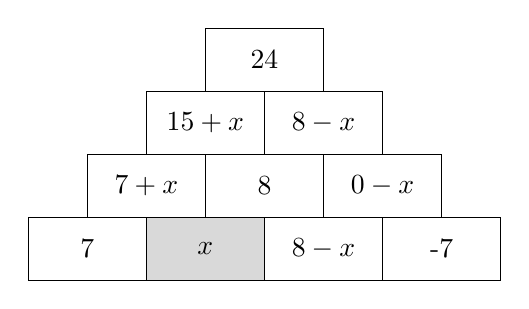
\begin{tikzpicture}
		\tikzstyle{brique}=[minimum width=1.5cm, minimum height=0.8cm,draw]
		\tikzstyle{brique_grise}=[minimum width=1.5cm, minimum height=0.8cm,draw,fill=gray!30]
		\node[brique] at (0,0) {  7 }; % gauche
		\node[brique_grise] at (1.5,0) {$x$};
		\node[brique] at (3,0) {$8-x$};
		\node[brique] at (4.5,0) { -7 };  % droite
		\node[brique] at (.75,.8) {$7+x$};
		\node[brique] at (2.25,.8) {  8 };  % milieu bas
		\node[brique] at (3.75,.8) {$0-x$};
		\node[brique] at (1.5,1.6) {$15+x$};
		\node[brique] at (3,1.6) {$8-x$};
		\node[brique] at (2.25,2.4) {24};
	\end{tikzpicture} 	
\end{center}
\end{minipage}


\end{correction}
\end{document}